\ifdefined\COMPILINGMAIN
% Main file is compiling this section, skip the preamble
\else
% Individual file compilation
\documentclass[11pt]{article}
% Geometry and page layout
\usepackage{geometry}
\geometry{verbose,tmargin=3.375cm,bmargin=2cm,lmargin=3.375cm,rmargin=3.375cm}

% Input encoding and font settings
\usepackage[utf8]{inputenc}

% other fonts
%Slightly more bold
% \usepackage{mlmodern}
% \usepackage[T1]{fontenc}

%Moder modern look
% \usepackage{libertine}
% \usepackage{libertinust1math}
% \usepackage[T1]{fontenc}

\usepackage{amsfonts, amsmath, amsthm, bbm, setspace}
\onehalfspacing
\usepackage{algorithm2e}
\usepackage{tcolorbox} % For the grey background
% Create a tcolorbox style for the algorithm
\tcbuselibrary{listingsutf8}
\tcbset{
    algobox/.style={
        colback=gray!3, % Background color
        colframe=black,  % Border color
        sharp corners,   % Square corners
        boxrule=0.5pt,   % Border thickness
        before skip=10pt, % Vertical spacing before box
        after skip=10pt,  % Vertical spacing after box
        width=\textwidth, % Box width
    }
}

% Adjust algorithm2e settings for a similar look
\SetKwInOut{Input}{Input}
\SetKwInOut{Result}{Result}
\SetKwFor{For}{for}{:}{end}

% Adjust settings for algorithm2e
\SetAlgoCaptionSeparator{.} % Separator for caption
\SetAlgoNlRelativeSize{-2}  % Adjust line number font size
\SetAlgoInsideSkip{2pt}    % Reduce space between lines
\SetAlCapSkip{0pt}         % Remove extra space after the caption
% Ensure captions are above algorithms
\SetAlgoCaptionLayout{center} % Center caption
% Adjust the style of the algorithm to remove bottom line
\RestyleAlgo{ruled}
\SetAlCapSkip{0.5em}       % Space after caption
\SetAlgoVlined              % Ensures no horizontal lines at the end

% Theorem and math environments
\newtheorem{assumption}{Assumption}
\newtheorem{lemma}{Lemma}
\newtheorem{theorem}{Theorem}

% New math commands
\newcommand{\npsym}{\mathrel{\ooalign{\raisebox{.6ex}{$>$}\cr\raisebox{-.6ex}{$<$}}}}

% Table formatting
\usepackage{booktabs, multirow, array, tabularx}
\newcolumntype{N}{>{\centering\arraybackslash}m{.85in}}

% Caption settings
\usepackage{caption}
\captionsetup{format=plain, font=footnotesize, labelfont=bf,width=3.5in}
\setlength{\abovecaptionskip}{3pt plus 3pt minus 3pt}

% Figures and floats setup
\usepackage{graphicx, adjustbox,subcaption}
\usepackage{floatrow}
\floatsetup[figure]{capposition=top}
\floatsetup[table]{capposition=top}
\renewcommand\thefigure{\thesection.\arabic{figure}}
% Path to figures
\graphicspath{{../Figures/}}
\usepackage{tikz} % TikZ for creating figures
% URLs and references and colors
\usepackage[dvipsnames]{xcolor}
\usepackage[hyphens]{url}
\usepackage{hyperref}
\hypersetup{
    colorlinks=true,
    citecolor=[HTML]{901A1E}, %KU red
    linkcolor=[HTML]{901A1E}, %KU red    
    filecolor=blue, 
    urlcolor=[HTML]{901A1E}, %KU red
    hyperindex=true,
    hyperfigures=true,
    hyperfootnotes=true,
}

% Biblatex settings for references
\usepackage[style=authoryear, dashed=false, backend=bibtex]{biblatex}
\addbibresource{../Ref.bib}

\renewbibmacro*{volume+number+eid}{%
  \printfield{volume}%
  \setunit*{\addcomma\space}%
  \printfield{number}%
  \setunit{\addcomma\space}%
  \printfield{eid}
}
\DeclareFieldFormat[article]{volume}{\bibstring{volume}~#1}
\DeclareFieldFormat[article]{number}{\bibstring{number}~#1}
\DefineBibliographyStrings{english}{volume = {Vol.}, number = {No.}}

% Author name formatting
\DeclareNameAlias{author}{last-first}
\renewcommand*{\finalnamedelim}{\addspace and\space}
\renewcommand*{\multinamedelim}{\addcomma\space}

% Footnotes and appendix setup
\usepackage[hang,flushmargin]{footmisc}
\usepackage[toc,page]{appendix}
\renewcommand\appendixtocname{Appendices}
\renewcommand\appendixpagename{Appendices}

%# Assumptions like theorems and corrolaries
% {
%   \theoremstyle{plain}
%   \newtheorem{assumption}{Assumption}
% }
% Title setup
\usepackage{titlepic}
\usepackage{titlesec}
\titleformat{\section}{\normalfont\Large\bfseries}{\thesection}{1em}{}[{\titlerule[0.1pt]}]
% no text above figures!!!!
\usepackage{placeins}

% Abbreviations (acronym package)
\usepackage{acro}
\acsetup{list/name = Abbreviations}
\DeclareAcronym{PML}{short=PML, long= Probabilistic Machine Learning}
\DeclareAcronym{NTR}{short=NTR, long=No-Trade Region}
\DeclareAcronym{MC}{short=MC, long=Monte Carlo}
\DeclareAcronym{QMC}{short=QMC, long=Quasi-Monte Carlo}
\DeclareAcronym{RQMC}{short=RQMC, long=Randomized Quasi-Monte Carlo}
\DeclareAcronym{LDS}{short = LDS, long = Low-Discrepancy Sequences}
\DeclareAcronym{LLN}{short = LLN, long = Law of Large Numbers}
\DeclareAcronym{GPR}{short = GPR, long = Gaussian process regression}
\DeclareAcronym{GP}{short = GP, long = Gaussian process}
\DeclareAcronym{ARD}{short = ARD, long = Automatic Relevance Detection}
\DeclareAcronym{LOVE}{short = LOVE, long = LanczOS Variance Estimates}
\DeclareAcronym{SKIP}{short = SKIP, long = Structured Kernel Interpolation for Products}
\DeclareAcronym{SGD}{short = SGD, long = Stochastic Gradient Descent}
\DeclareAcronym{DP}{short = DP, long = Dynamic Programming}
\DeclareAcronym{MPT}{short=MPT, long=Modern Portfolio Theory}


% Conditional macro for compiling individual files
\ifdefined\COMPILINGMAIN
% Define settings when compiling the main document
\else
% Define minimal preamble for individual file compilation
\usepackage{geometry}
\geometry{verbose,tmargin=3.375cm,bmargin=2cm,lmargin=3.375cm,rmargin=3.375cm}
\fi

\AtBeginDocument{%
    \renewcommand{\contentsname}{Table of Contents}
    \renewcommand{\abstractname}{Abstract}
}
\setlength\parindent{11pt}
% Define the macro for compiling the main file
%\def\COMPILINGMAIN{}  % Include the main preamble
\begin{document}
\fi

\section{Numerical implementation details} \label{Section: Implmentation-details}
This section covers detail regarding the solution algorithm and numerical implementation.
Each method is presented in a separate subsection, and the final solution algorithm is presented in the last subsection,
which combines each of the methods. These span points sampling, numerical integration techniques, function approximation methods
and solution techniques specific to this class of problemns.
\subsection{Numerical integration} \label{Subsection: NumericalIntegration}
Consider the basic problem with proportional transaction costs, basic risky assets and a risk-free asset and no stochastic parameters.
We need to evaluate the expectation of the value function:
$\mathbb{E} \left[ v_{t+\Delta t} (\mathbf{x}_{t+\Delta t }  ) \right]$.
In order to compue this expectation, we need to evaluate the integral:
\begin{equation}
  \mathbb{E}_{t} \left[ \pi_{t+1}^{1-\gamma} v_{t+1} (x_{t+1}) \right] = \int \pi_{t+1}^{1-\gamma} v_{t+1} (x_{t+1}) f(R_{t+1}), d R_{t+1}
\end{equation}
where $f(R_{t+1})$ is the probability density function of the risky asset returns. If we look at the case of stochastic parameters, 
would need to evaluate the conditional expectation with regard to these aswell, given some distributional assumption on the parameters.
The integral can be computed using Monte-carlo methods
or by using quadrature rules.
\subsubsection{Gauss-Hermite quadrature} \label{Subsection: Gauss-Hermite}
Gaussian quadrature is a numerical integration method based on approximation and interpolation theory.
Gaussian quadrature can be used to approximate integrals using the following form, \textcite{Judd1998Book}:
\begin{equation}
  \int_{a}^{b} f(x) w(x) dx \approx \sum_{i=1}^{n} \omega_{i} f(x_{i}),
\end{equation}
Where $\omega_i$ are quadrature weights, $x_i$ are quadrature nodes and $w(x)$ is a weighting function.
This approximation is exact when $f(x)$ is a polynomial of degree $2n-1$ or less.
Then we can approximate the integral using $n$ points $x_i$ and $n$ weights $\omega_i$.
There are many different Gaussian quadrature schemes, with differering intervals $[a,b]$ and weighting functions $w(x)$.
We consider the use of a Gauss-Hermite quadrature rule, for a comprehensive review on Gaussian quadrature rules, see \textcite{Judd1998Book}.
Gauss-Hermite quadrature is used to approximate integrals of the form:
\begin{equation}
  \int_{-\infty}^{\infty} f(x) e^{-x^{2}} dx \approx \sum_{i=1}^{n} \omega_{i} f(x_{i}) + \frac{n! \sqrt{\pi}}{2^{n}} 
  \cdot \frac{f^{(2n) }(\zeta )}{(2n)!},
\end{equation}
Where $\zeta \in (-\infty , \infty)$.
If a random variable $X$ is normally distributed, i.e  $X \sim \mathcal{N}(\mu , \sigma^{2})$,
then we can compute the expectation, $\mathbb{E}[f(X)]$, which is given by:
\begin{equation}
  \mathbb{E} [f(X)] =  \frac{1}{\sqrt{2\pi \sigma^{2}} } \int_{-\infty}^{\infty} f(x)  e^{-\frac{(x-\mu)^{2}}{2\sigma^{2}}} dx 
\end{equation}
Using a change of variables $y = \frac{x-\mu}{\sqrt{2}\sigma}$, then we can rewrite the expectation on the form of the Gauss-Hermite quadrature rule:
\begin{align}
  \mathbb{E} [f(X)] &=  \frac{1}{\sqrt{2\pi \sigma^{2}} } \int_{-\infty}^{\infty} f( \sqrt{2} \sigma y + \mu)  e^{-y^{2}} \sqrt{2} \sigma dy \\
  &= \frac{1}{\sqrt{\pi}} \int_{-\infty}^{\infty} e^{-y^{2}} f( \sqrt{2} \sigma y + \mu) dy \\
  &\approx \frac{1}{\sqrt{\pi}} \sum_{i=1}^{n} \omega_{i} f( \sqrt{2} \sigma x_{i} + \mu)
\end{align}
Where $\omega_i$ are the quadrature weights, $x_i$ are the quadrature nodes over the interval $(-\infty , \infty)$.\\
When $X$ is log-normal, i.e $\log X \sim \mathcal{N}(\mu , \sigma^{2})$, then we can use a variable change once again:
$X = e^{Y}$ and $Y \sim \mathcal{N}(\mu , \sigma^{2})$. Then we can rewrite the expectation as:
\begin{equation}
  \mathbb{E} [ f(X) ] = \mathbb{E} [ f(e^{Y}) ] \approx \pi^{-\frac{1}{2}} \sum{n}_{i=1} \omega_i f \left( e^{ \sqrt{2} \sigma x_{i} + \mu } \right)
\end{equation}

If we want to extend this framework to multiple dimensions we can use product rules as noted by \textcite{CaiJuddXu2013}.
Consider $Y$ which is multivariate normal, i.e $Y \sim \mathcal{N}(\boldsymbol{\mu} , \Sigma)$,
where $\mu$ is the drift vector and $\Sigma$ is the covariance matrix.
Let $L$ be a lower-triangular matrix such that $LL^{\top} = \Sigma$ (Cholesky factorisation).
Then we have that:
\begin{align}
  \mathbb{E}\{f(Y)\} & = \left( (2\pi)^d \det(\Sigma) \right)^{-\frac{1}{2}} \int_{\mathbb{R}^d} f(y) \, e^{-\frac{1}{2}(y - \mu)^{\top} \Sigma^{-1} (y - \mu)} \, dy \\
  & = \left( (2\pi)^d \det(L)^2 \right)^{-\frac{1}{2}} \int_{\mathbb{R}^d} f\left(\sqrt{2} L y + \mu\right) \, e^{-\frac{1}{2} y^{\top} y} \, dy \\
  & \approx \pi^{-\frac{d}{2}} \sum_{i_1=1}^n \cdots \sum_{i_d=1}^n \omega_{i_1} \cdots \omega_{i_d} \, f
  \bigg(\sqrt{2} L_{1,1} y_{i_1} + \mu_1, \;
  \notag \\
  & \quad \sqrt{2} (L_{2,1} y_{i_1} + L_{2,2} y_{i_2}) + \mu_2, \;
  \ldots, \;
  \sqrt{2} \big(\sum_{j=1}^d L_{d,j} y_{i_j}\big) + \mu_d
  \bigg) 
  \end{align}
Where $d$ refers to the number of dimensions, $n$ is the number of quadrature points, $\omega_i$ are the quadrature weights and $y_i$ are the quadrature nodes.
$L_{i,j}$ is the $i$th row and $j$th column of the Cholesky factorisation matrix $L$. $\det$ is the matrix determinant.
We note that the use of product rules suffers from the curse of dimensionality, 
as the complexity scales exponentionally with the number of dimensions. This is because the quadrature points with the product rule,
normally use a tensor product grid, which is constructed using the Cartesian product of the quadrature points in each dimension.
We can use sparse grid methods to partially tackle this. One common method  is the Smolyak method, \textcite{smolyak1963}.
Smolyaks sparse grid method approximates multidimensional integrals, over dimesion $d$
while limiting the amount of points used. The method is composed of the following:
\begin{enumerate}
  \item \textbf{Univariate Quadrature Rules}: Each dimension of the integration domain is assigned a univariate quadrature rule, which provides both nodes (quadrature points) and weights for numerical integration in that dimension. The accuracy of each rule is determined by its \textit{level}, denoted by \( i_d \) for each dimension \( d \). The level determines the number of quadrature points in that dimension, which improves the accuracy of the quadrature rule. 
  
  \item \textbf{Approximation Level (\( \mu \))}: The accuracy of the Smolyak sparse grid is controlled by the \textit{approximation level} \( \mu \). This parameter sets a limit on the sum of levels across all dimensions, controlling the total number of grid points. Higher values of \( \mu \) result in more accurate approximations but increase computational complexity.

  \item \textbf{Multi-Index and Combination of Levels}: In a \( d \)-dimensional integral, the Smolyak method uses a \textit{multi-index} \( i = (i_1, i_2, \dots, i_d) \) to represent the level of the quadrature rule in each dimension. The multi-index specifies a unique combination of quadrature levels for each dimension, where \( i_d \) denotes the level for dimension \( d \). To construct a sparse grid, Smolyak’s method restricts the sum of these levels using the following condition:
  \[
  d \leq i_1 + i_2 + \dots + i_d \leq d +  \mu
  \]
  This constraint on the sum of levels, reduces the number of tensor products. We denote the sum of multi indicies: $\lvert i \rvert = i_1 + i_2 + \dots i_d$.

  \item \textbf{Tensor Product of Univariate Rules}: The Smolyak grid is formed by taking the \textit{tensor product} of univariate quadrature rules that satisfy the multi-index constraint. Each univariate quadrature rule, represented by \( Q_{i_d} \) at level \( i_d \) in dimension \( d \), is combined across dimensions according to the set of multi-indices \( i \). This combination is given by:
  \[
  A(\mu, d) = \sum_{d \leq |i| \leq d + \mu} (-1)^{\mu + d - |i|} \binom{d - 1}{\mu + d - 1 - |i|} \bigotimes_{d=1}^d Q_{i_d}
  \]
  where:
  \begin{itemize}
      \item \( Q_{i_d} \) is the univariate quadrature rule at level \( i_d \) in dimension \( d \),
      \item \( \bigotimes \) denotes the tensor product, and
      \item \( \binom{d - 1}{\mu + d - 1 - |i|} \) is a combinatorial coefficient that assigns weights to each tensor product, for accurate integration up to the specified approximation level \( \mu \).
  \end{itemize} 
\end{enumerate}
By resticting the multi indicies \( i \) with the approximation level \( \mu \), the Smolyak method reduces 
the number of points needed for numerical integration in higher dimensions.
Tensor grid methods grows exponentially with the number of dimensions \( d \), the Smolyak grid grows polynomially, \textcite{judd2014smolyak},
hence it directly combats the curse of dimensionality. For more on this see \textcite{smolyak1963}, \textcite{judd2014smolyak} and
\textcite{horneff2016efficient}. 

\subsubsection{Monte Carlo integration (MC)} \label{Subsection: MC}
Monte Carlo integration is a numerical integration method based on \textit{sampling}, as opposed to
quadrature rules which are based on interpolation. \\
The convergence of Monte Carlo integration is generally slower
than some quadrature methods; however, its convergence rate is independent of
the dimensionality of the integral, making it well-suited for high-dimensional problems.
Monte Carlo integration breaks the curse of dimensionality.
\ac{MC} integration is based on random sampling\footnote{Strictly speaking the samples are not random, but pseudo-random, meaning that deterministic samples are used, which appear random. For more in this see \textcite{Judd1998Book} or  \textcite{Glasserman2004MC}}
over the domain of the integral, and then computing the sample average of the function to be integrated.
Assume we wish to approximate the $d$-dimensional integral:
\begin{equation} \label{eq: MC-integral}
  I = \int_{\Omega} f(\mathbf{x}) g(\mathbf{x}) d\mathbf{x} = \mathbb{E}[f(\mathbf{x})],
\end{equation}
where \( g(\mathbf{x}) \) is the probability density function of the random variable \( \mathbf{x} \) over its support \( \Omega \), we approximate \( I \) as:
\begin{equation} \label{eq: MC-integralapproximation}
  Q_N = \frac{1}{N} \sum_{i=1}^{N} f(\mathbf{X}_i),
\end{equation}
where \( \mathbf{X}_i \) are independent samples drawn from \( g(\mathbf{x}) \).
The procedure is then:
\begin{enumerate}
  \item Sample \( N \) points \( \mathbf{x}_1, \ldots, \mathbf{x}_N \) from \( g(\mathbf{x}) \).
  \item Approximate the expectation \( \mathbb{E}[f(\mathbf{x})] \) by the sample average:
\end{enumerate}
\[
I \approx Q_{N} = \frac{1}{N} \sum_{i=1}^{N} f(\mathbf{x}_{i}).
\]
The Law of Large Numbers ensures that the sample average converges to the mean as \( N \to \infty \):
\[
\lim_{{N \to \infty}} Q_{N} = \mathbb{E}[f(\mathbf{x})] = I.
\]
And by the Central Limit Theorem, we have:
\[
\sqrt{N} \left( Q_N - I \right) \xrightarrow{d} N\left(0, \sigma^2 \right),
\]
where \( \sigma^2 = \operatorname{Var}[f(\mathbf{x})] \) does not depend on \( N \) or \( d \). 
The standard error of \( Q_N \) is:
\[
\sigma_{Q_N} = \frac{\sigma}{\sqrt{N}}.
\]
The convergence rate of \( 1/\sqrt{N} \) is independent of the dimension. 
\subsubsection{Quasi-Monte Carlo integration (QMC)} \label{Subsubsection: QMC}
Quasi-Monte Carlo integration substitutes the 'random' samples in Monte Carlo integration 
with specific deterministic sequences such as equidistributred sequences, \ac{LDS} or Lattice point rules etc.
We will focus on the use of low discrepancy sequences. For a comprehesive review of sequences and rules see \textcite{Judd1998Book}.\\
\ac{LDS} are deterministic sequences which cover the domain of the integral more evenly than random samples. 
Discrepancy is in this case a measure of deviation from perfect uniformity over the domain of the integral.
Thus to go from MC in \eqref{eq: MC-integralapproximation} to QMC, we replace the random samples $\mathbf{X}_i$ with \ac{LDS} samples.
We note that the sampling of the QMC is now dependent on the dimensionality of the integral, as opposed to MC,
as the LDS samples have to be drawn with respect to the dimensionality of the integral.

We consider two different types of \ac{LDS} sequences, the Halton sequence and the Sobol sequence.
Both sequences are popular \ac{LDS} sequences,
which are used in \ac{QMC} applications, \autocite{Glasserman2004MC}.

The convergence rate of \ac{QMC} is:
\begin{equation} \label{eq: QMC-convergence}
  \frac{\left( \log N \right)^{d}}{N}
\end{equation}
Hence QMC is generally faster than MC, e.g $\frac{\left( \log N \right)^{d}}{N} < \frac{1}{\sqrt{N}}$ for large $N$ and small $d$.
We note that as dimensionality $d$ increases, the quality of the Halton sequence decreases, as the dimensions become more correlated, \textcite{Glasserman2004MC}.
Specifically the Halton seuqnce will produce diagonal points when projected onto a 2D plane.
This is displayed in figure \ref{fig: Sampling_comparison_MC_D1D2}. 
We therefore prefer the Sobol sequence when the dimensionality is sufficiently high,
and as not to complicate matters, also use the Sobol sequence in lower dimensions, when \ac{QMC} schemes are used.
Figures below shows Random samples, Halton samples and Sobol samples in 2d.
Second figure shows the same in 18 dimensions. Halton shows that dimension 17 and 18 are correlated.
\begin{figure}[h!]
  \begin{center}
  \caption{Comparison of sample generation for Monte Carlo and Quasi-Monte Carlo} 
  \label{fig: Sampling_comparison_MC_D1D2}
  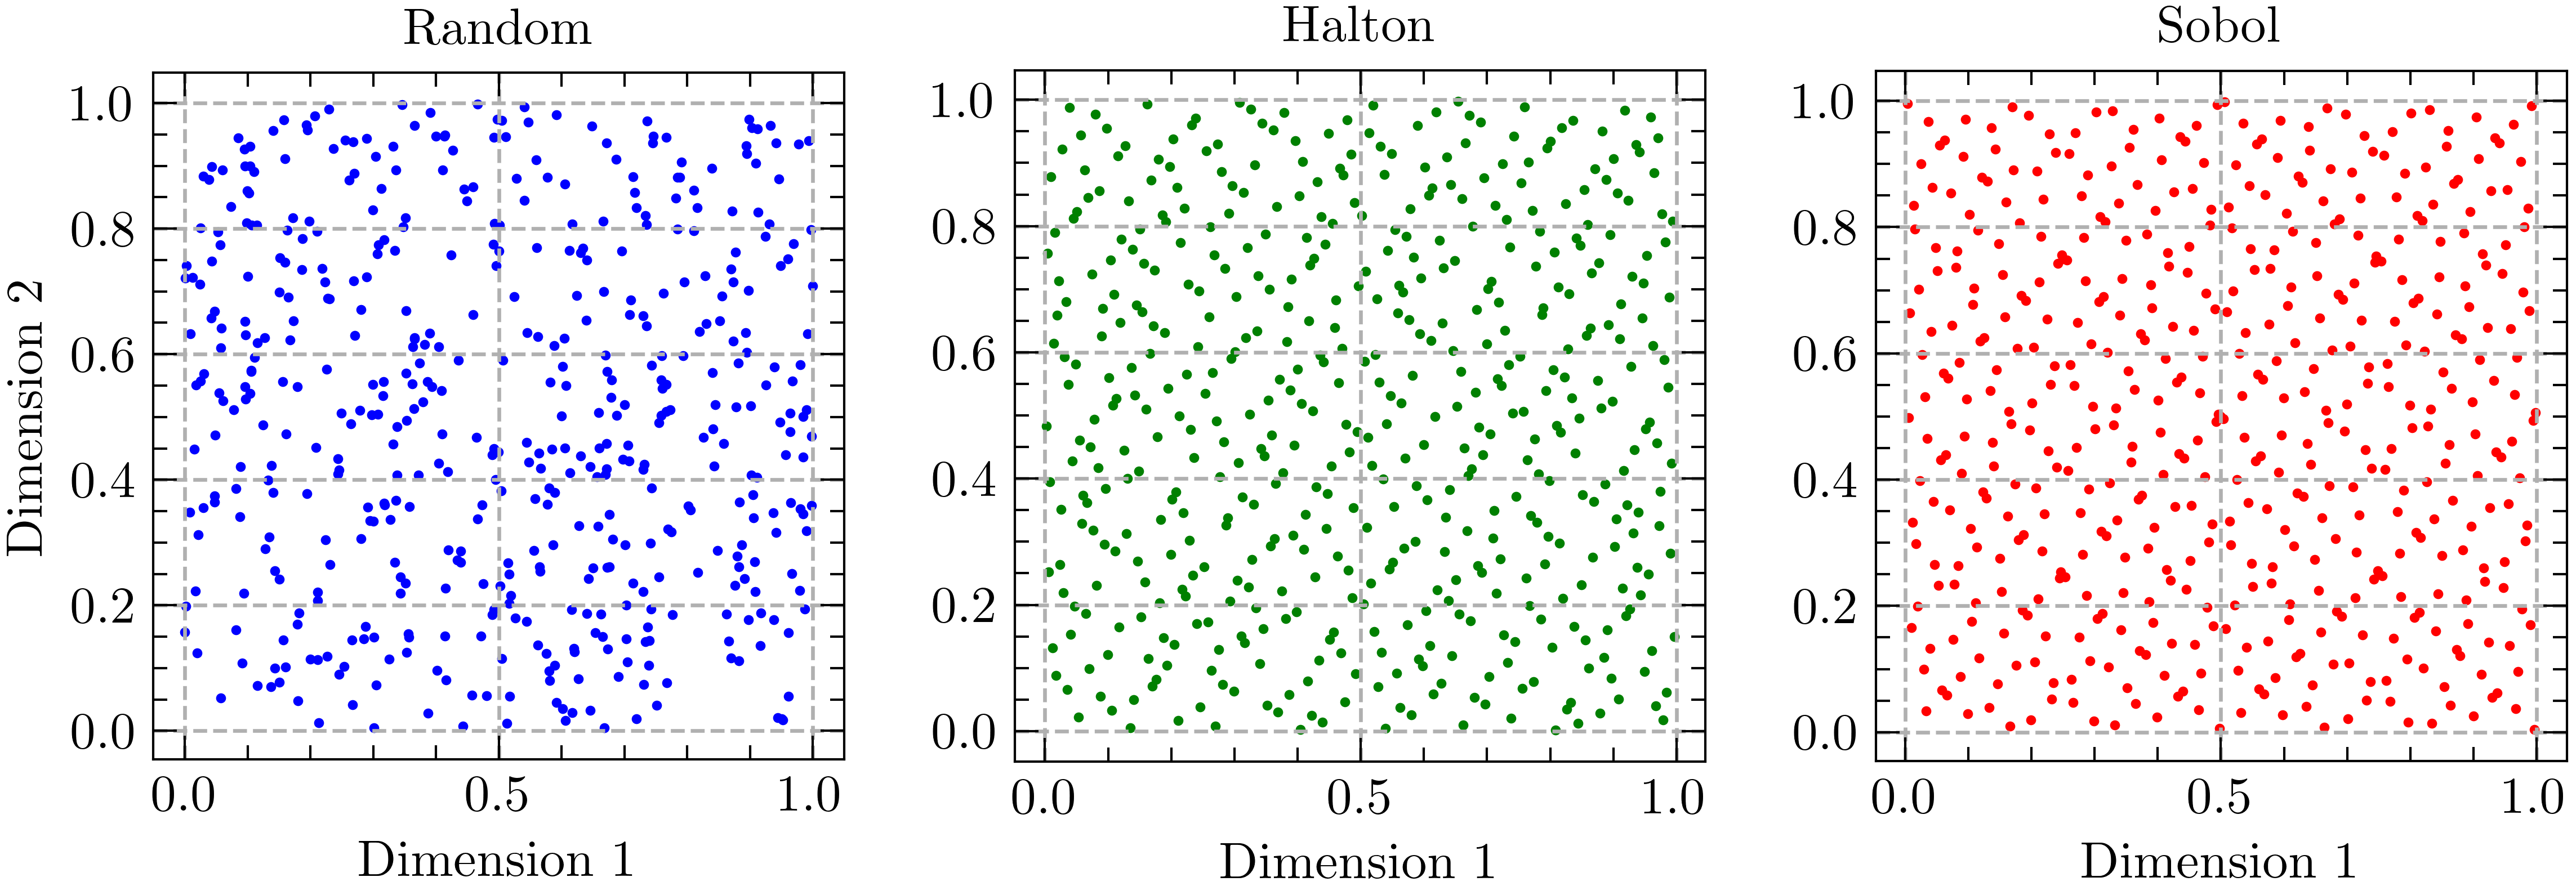
\includegraphics[width=\textwidth]{sampling_comparison_d1_d2.png}
  \end{center}
  \floatfoot{\textbf{Note:} 
  Each sequence was generated using $N = 500$ samples and $d = 2$ dimensions.}
\end{figure}

\begin{figure}[h!]
  \begin{center}
  \caption{Comparison of sample generation for Monte Carlo and Quasi-Monte Carlo with increased dimensionality} 
  \label{fig: Sampling_comparison_MC_D17D18}
  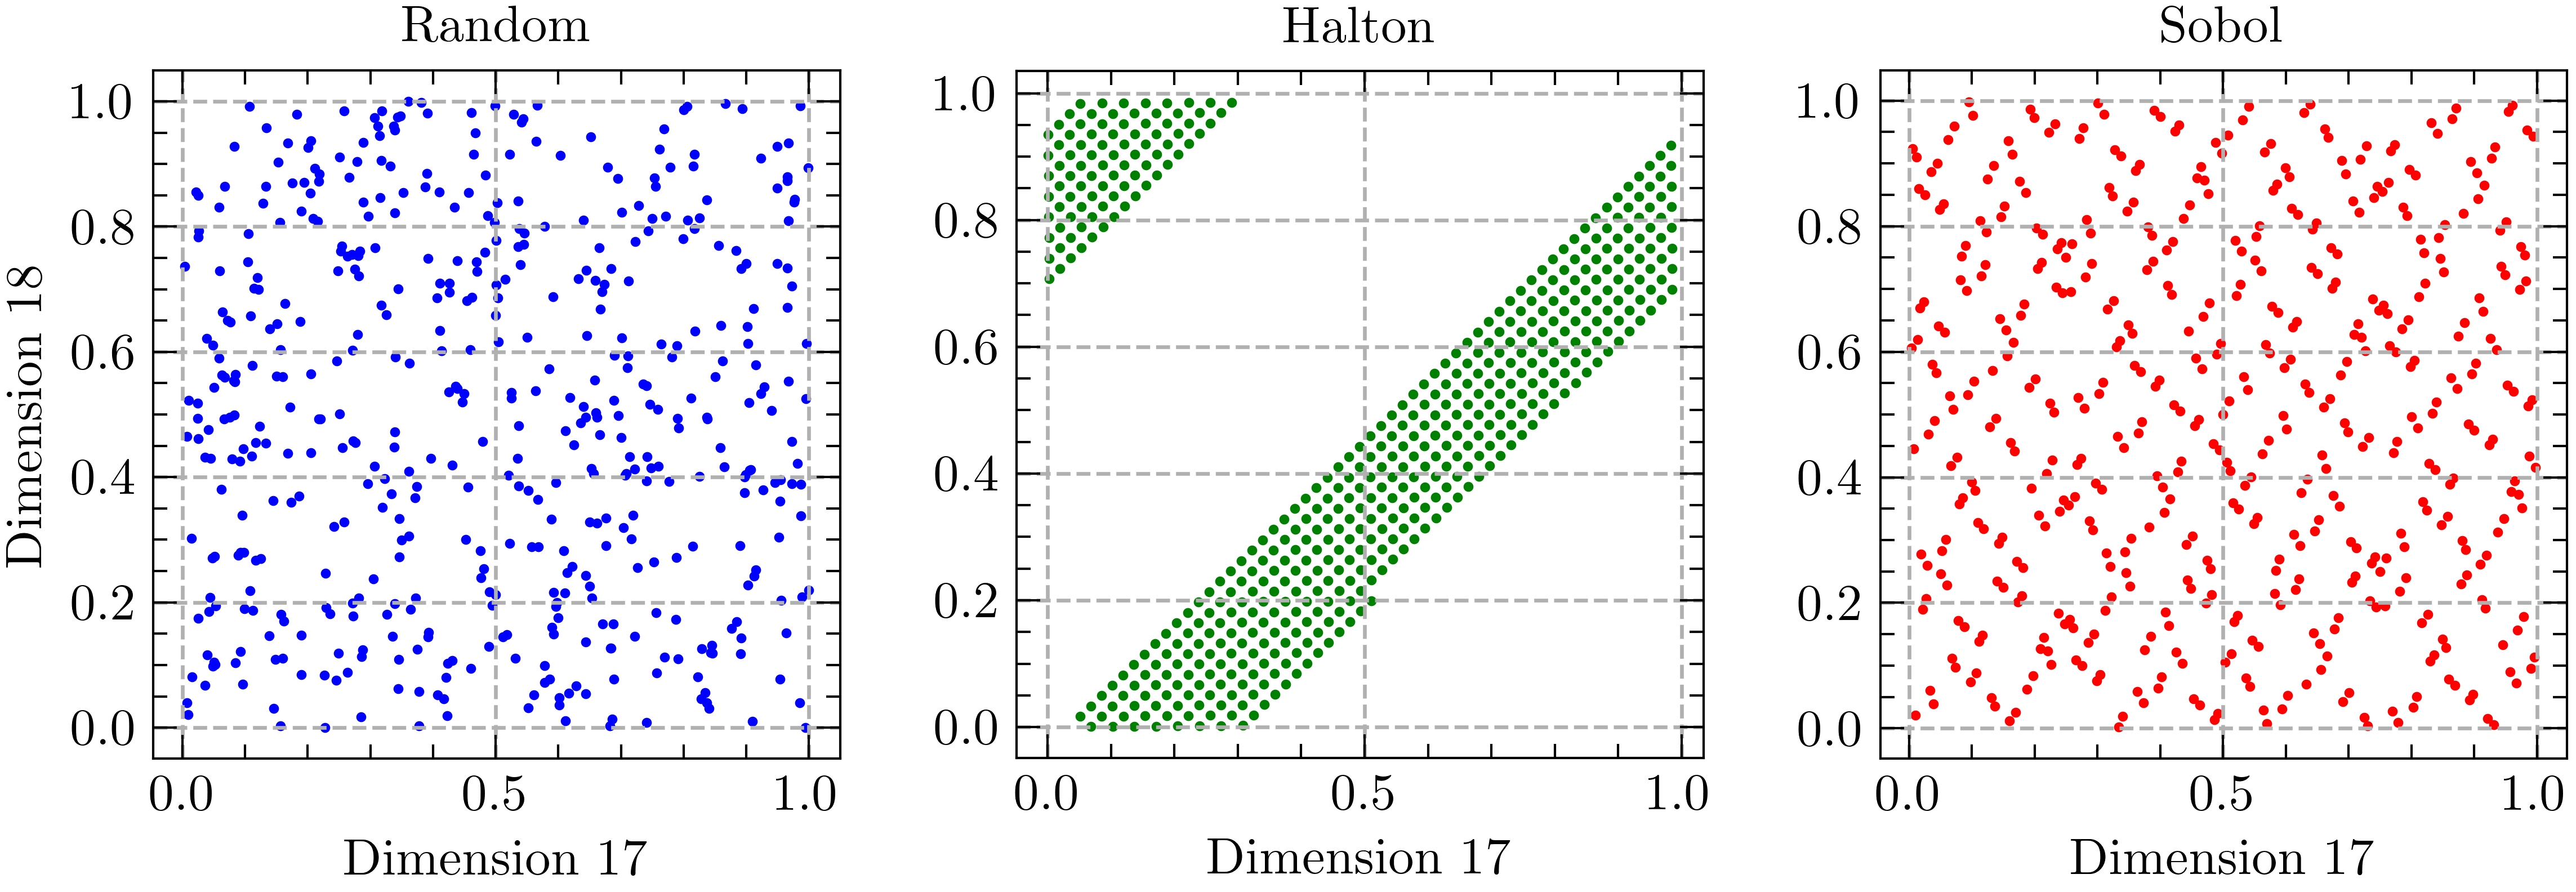
\includegraphics[width=\textwidth]{sampling_comparison_d17_d18.png}
  \end{center}
  \floatfoot{\textbf{Note:} 
  Each sequence was generated using $N = 500$ samples and $d = 18$ dimensions.}
\end{figure}
QMC is generally found to be more efficient than MC, as noted by \textcite{Glasserman2004MC}, \textcite{Judd1998Book},
and notably Glasserman find that dimensionality has to be quite large before the Monte Carlo method is favorable to the quasi Monte Carlo method.
Furthermore Glasserman find that while we generally might assume that $N$ must by increase a lot when $d$ is increased, this is not
always the case in classic financial applications, as the integrals employed in these examples can often
be approximated by integrals of much lower dimension. QMC therefore performs better than to be expected.

However we note that \ac{QMC} lacks a straightforward variance estimator,
a feature recovered through \textit{randomized QMC}, which will be discussed in the next section.

\subsubsection{Randomized Quasi-Monte carlo integration (RQMC)} \label{Subsection: RQMC}
Randomized quasi-Monte Carlo integration (RQMC) is a combination of \ac{QMC} and \ac{MC} integration.
We consider the the QMC integral, i.e the equaiton of \eqref{eq: MC-integralapproximation}, using an \ac{LDS} sequence.
The point of \ac{RQMC} is then to introduce randomness to the sequence: $P_{n} = \{ x_1 , \ldots , x_n \}$.
We will cover the most simple case, \textit{Random shift} and \textit{Scrambling} methods, however for a comprehensive review of randomization methods see \textcite{Glasserman2004MC}.
The most simple method of randomizing $P_n$ is to add a \textit{random shift} to each point in the sequence, using
random numbers drawn from a uniform distribution of the same dimensionality as the sequence, wrapped to the interval of $P_n$.
Hence if $x_{i} \in [0,1)^{d}$ then we add a random shift $u_{i} \operatorname{mod} 1$, where
$\operatorname{mod} 1$ keeps the shift within the interval $[0,1)$. 
A major disadvantage of the random shift is that is changes the discrepancy properties of the sequence,
and hence the quality of the sequence is lost.\\
Scrambled nets is a method of randomization which can be applied to \ac{LDS} sequences specifically.
Scrambling works by applying a sequence of random permutations to the 
digits in the base-b representation of each coordinate in the \ac{LDS}.
Each digit is permuted based on the values of the digits that came before it. 
This structure retains the low-discrepancy properties 
while introducing a controlled level of randomness, 
which enables the calculation of variance for RQMC estimates.
In multi-dimensional settings, this scrambling is applied independently to each coordinate of the sequence, allowing us to estimate variance across the entire space.
Scrambling the Sobol sequence has been found to be particularily effective in financial applications,
as noted by \textcite{Scramble2023}. QMC is generally more efficient than MC, and RQMC increases the rate of converence of QMC
and allows for the estimation of variance.  
\subsection{Value function approximation}
This section covers the necessary function approximation methods used in the solution algorithm.
We will cover the use of \ac{GPR} and Baysian optimization, in order to maximize the value function of the dynamic portfolio allocation problem. 


\subsubsection{Gaussian process regressions (GPR)} \label{Subsubsection: GPR}
A \ac{GP} is a probabilistic model that defines a distribution over functions used to make predictions based on available data. 
It is specified by two functions: the mean function and the covariance function, also called the kernel. 
The mean function, \( m(\mathbf{x}) \), represents the expected value of the function at a given input \( \mathbf{x} \), 
and the covariance function, \( k(\mathbf{x}, \mathbf{x}') \), 
captures the covariance between function values at different input points \( \mathbf{x} \) and \( \mathbf{x}' \).
In a \ac{GP}, any finite set of input points \( \mathbf{X} = (\mathbf{x}_1, \dots, \mathbf{x}_N) \) within the domain \( \mathbb{R}^d \) 
results in the function values \( \mathbf{f} = (f(\mathbf{x}_1), \dots, f(\mathbf{x}_N)) \) having a joint multivariate Gaussian distribution.
This property enables a GP to provide a prior distribution over functions based on the defined mean and covariance.

We use \ac{GPR} to estimate the value function in the dynamic portfolio allocation problem,
when we are not at the terminal period, i.e., \( t < T \), following \textcite{Scheidegger2023}.
The \ac{GP} is formulated by the previously mentioned mean and covariance functions:
\begin{equation} \label{eq: GP-definition}
  f(\mathbf{x}) \sim \mathcal{GP}(m(\mathbf{x}), k(\mathbf{x}, \mathbf{x}')),
\end{equation}
The covariance kernel function \( k(\mathbf{x}, \mathbf{x}') \) can be any Mercer kernel, i.e., positive definite \autocite{MurphyBook2023}.
Common kernel choices include the Radial Basis Function (RBF) kernel, the Matern kernel, and the Exponential kernel.
We employ a Matern kernel, which, depending on the parameter \( \nu \), 
can be a generalization of the RBF kernel or the Exponential kernel. This choice follows \textcite{Scheidegger2023}.
The Matern kernel is given by:
\begin{equation} \label{eq: Matern-kernel}
  k_{\text{Matern}}(\mathbf{x} , \mathbf{x}') = \frac{2^{1-\nu}}{\Gamma(\nu)}  \left( \frac{\sqrt{2 \nu} \| \mathbf{x} - \mathbf{x}' \|_{2}}{\ell} \right) K_{\nu} \left( \frac{\sqrt{2 \nu} \| \mathbf{x} - \mathbf{x}' \|_{2}}{\ell} \right),
\end{equation}
where \( \| \cdot \|_{2} \) is the Euclidean norm, \( \Gamma \) is the gamma function, and \( K_{\nu} \) is the modified Bessel function.
The length scale \( \ell \) and smoothness parameter \( \nu \) are both positive. As \( \nu \to \infty \), the Matern kernel converges to the RBF kernel \autocite{Gonzalvez2019}.
Functions from this class are \( k \)-times differentiable when \( \nu > k \).
When \( \nu = 1/2 \), the Matern kernel corresponds to the Ornstein-Uhlenbeck process \autocite{MurphyBook2023},
which is commonly used in financial applications, such as models of interest rates \autocite{Glasserman2004MC}. 

Consider a training dataset \( \{ \mathbf{X}, \mathbf{y} \} \)
with \( N \) states \( \mathbf{x}_{i} \) and observed values \( \mathbf{y} \). 
We assume that the observations \( \mathbf{y} \) are generated by an unknown function \( f \), such that
\[
y_i = f(\mathbf{x}_i) + \varepsilon_{i}, \quad \varepsilon_{i} \sim \mathcal{N}(0, \sigma^{2}_{\varepsilon}),
\]
where \( \sigma^{2}_{\varepsilon} \) represents the observational noise\footnote{The noise assumption implies that the GP model does not interpolate the data but rather fits a smooth function. 
This results in computational costs of \( O(N) \) for the mean prediction and \( O(N^2) \) for the variance prediction. For more details, see \autocite{MurphyBook2023}.}.
The goal is to train a \ac{GP} on this dataset and then use it to predict the value function at a new state \( \mathbf{x}_{*} \),
yielding a new predicted output \( f_{*} \).

The training observations \( \mathbf{y} \) and the predicted noise-free function \( f_{*} \) 
have a joint Gaussian distribution:
\begin{equation}\label{eq: GP-distribution}
  \begin{bmatrix}
    \mathbf{y} \\
    \mathbf{f}_{*}
  \end{bmatrix}
  \sim 
  \mathcal{N} \left( \mathbf{0},
                \begin{bmatrix}
                  k(\mathbf{X}, \mathbf{X}) + \sigma^{2}_{\varepsilon} \mathbf{I} & k(\mathbf{X}, \mathbf{x}_{*}) \\
                  k(\mathbf{x}_{*}, \mathbf{X}) & k(\mathbf{x}_{*}, \mathbf{x}_{*})
                \end{bmatrix}
              \right)
\end{equation}
Here i have assumed a zero mean function\footnote{Zero mean ... XXXX}, and the kernel function is the Matern kernel.
The posterior distribution of the predicted value function \( f_{*} \) given the training data is then a multivariate normal \autocite{MurphyBook2023},
with mean:
\begin{equation} \label{eq: GP-pred-mean}
  \tilde{\mu}(\mathbf{x}) = k(\mathbf{x}_{*}, \mathbf{X}) [k(\mathbf{X}, \mathbf{X}) + \sigma^{2}_{\varepsilon} \mathbf{I}]^{-1} \mathbf{y},
\end{equation}
And covariance:
\begin{equation} \label{eq: GP-pred-covariance}
 \tilde{k} (\mathbf{x}_* , \mathbf{x}_{*}^{'}) = 
 k (\mathbf{x}_* , \mathbf{x}_{*}^{'}) - 
 k (\mathbf{x}_* , \mathbf{X}) 
  [k (\mathbf{X} , \mathbf{X}) + \sigma^{2}_{\varepsilon} \mathbf{I}]^{-1}
  k (\mathbf{X} , \mathbf{x}_{*}^{'})
\end{equation}
Therefore in order to predict the value function at a new state $\mathbf{x}_{*}$, we need to compute the mean and covariance.
This step is computationally burdensome as we have to compute the four covariance matrices in the joint distribution \eqref{eq: GP-distribution}.
Afterwards we can compute predictions using the mean function \eqref{eq: GP-pred-mean} and the covariance function \eqref{eq: GP-pred-covariance}
can be used to compute error bands on our predictions. 

As noted, training and predicting with a \ac{GP} is computationally expensive. I will therefore introduce
the methods employed to reduce the computational burden of the \ac{GP}.

We use automatic relevance detection (ARD) which is a modification to the Matern kernel to use
a length scale for each dimension, $\ell_{i}$. Dimensions with low impact has a high length scale, and are effectively ignored.
Note that this is not the same as Lasso, as these coefficients are not set to $0$.

We use \ac{LOVE} to reduce the computational burden of estimating the variance of the \ac{GP}.

We use \ac{SKIP} to reduce the computational burden of computen the matrices in the joint distribution \eqref{eq: GP-distribution}.

\textbf{Use LancZos Variance Estimate (Love) and SKIP to reduce computational burden.}\\
Here is the documentation in my package 
\url{https://docs.gpytorch.ai/en/stable/examples/02_Scalable_Exact_GPs/index.html} 

And here is a paper on the subject \url{https://arxiv.org/pdf/1803.06058}.
\subsubsection{Strategic point sampling} \label{Subsection: Sample}


\begin{figure}[h!]
  \begin{center}
  \caption{A designed sampling strategy} 
  \label{fig: Designed_sampling_strategy}
  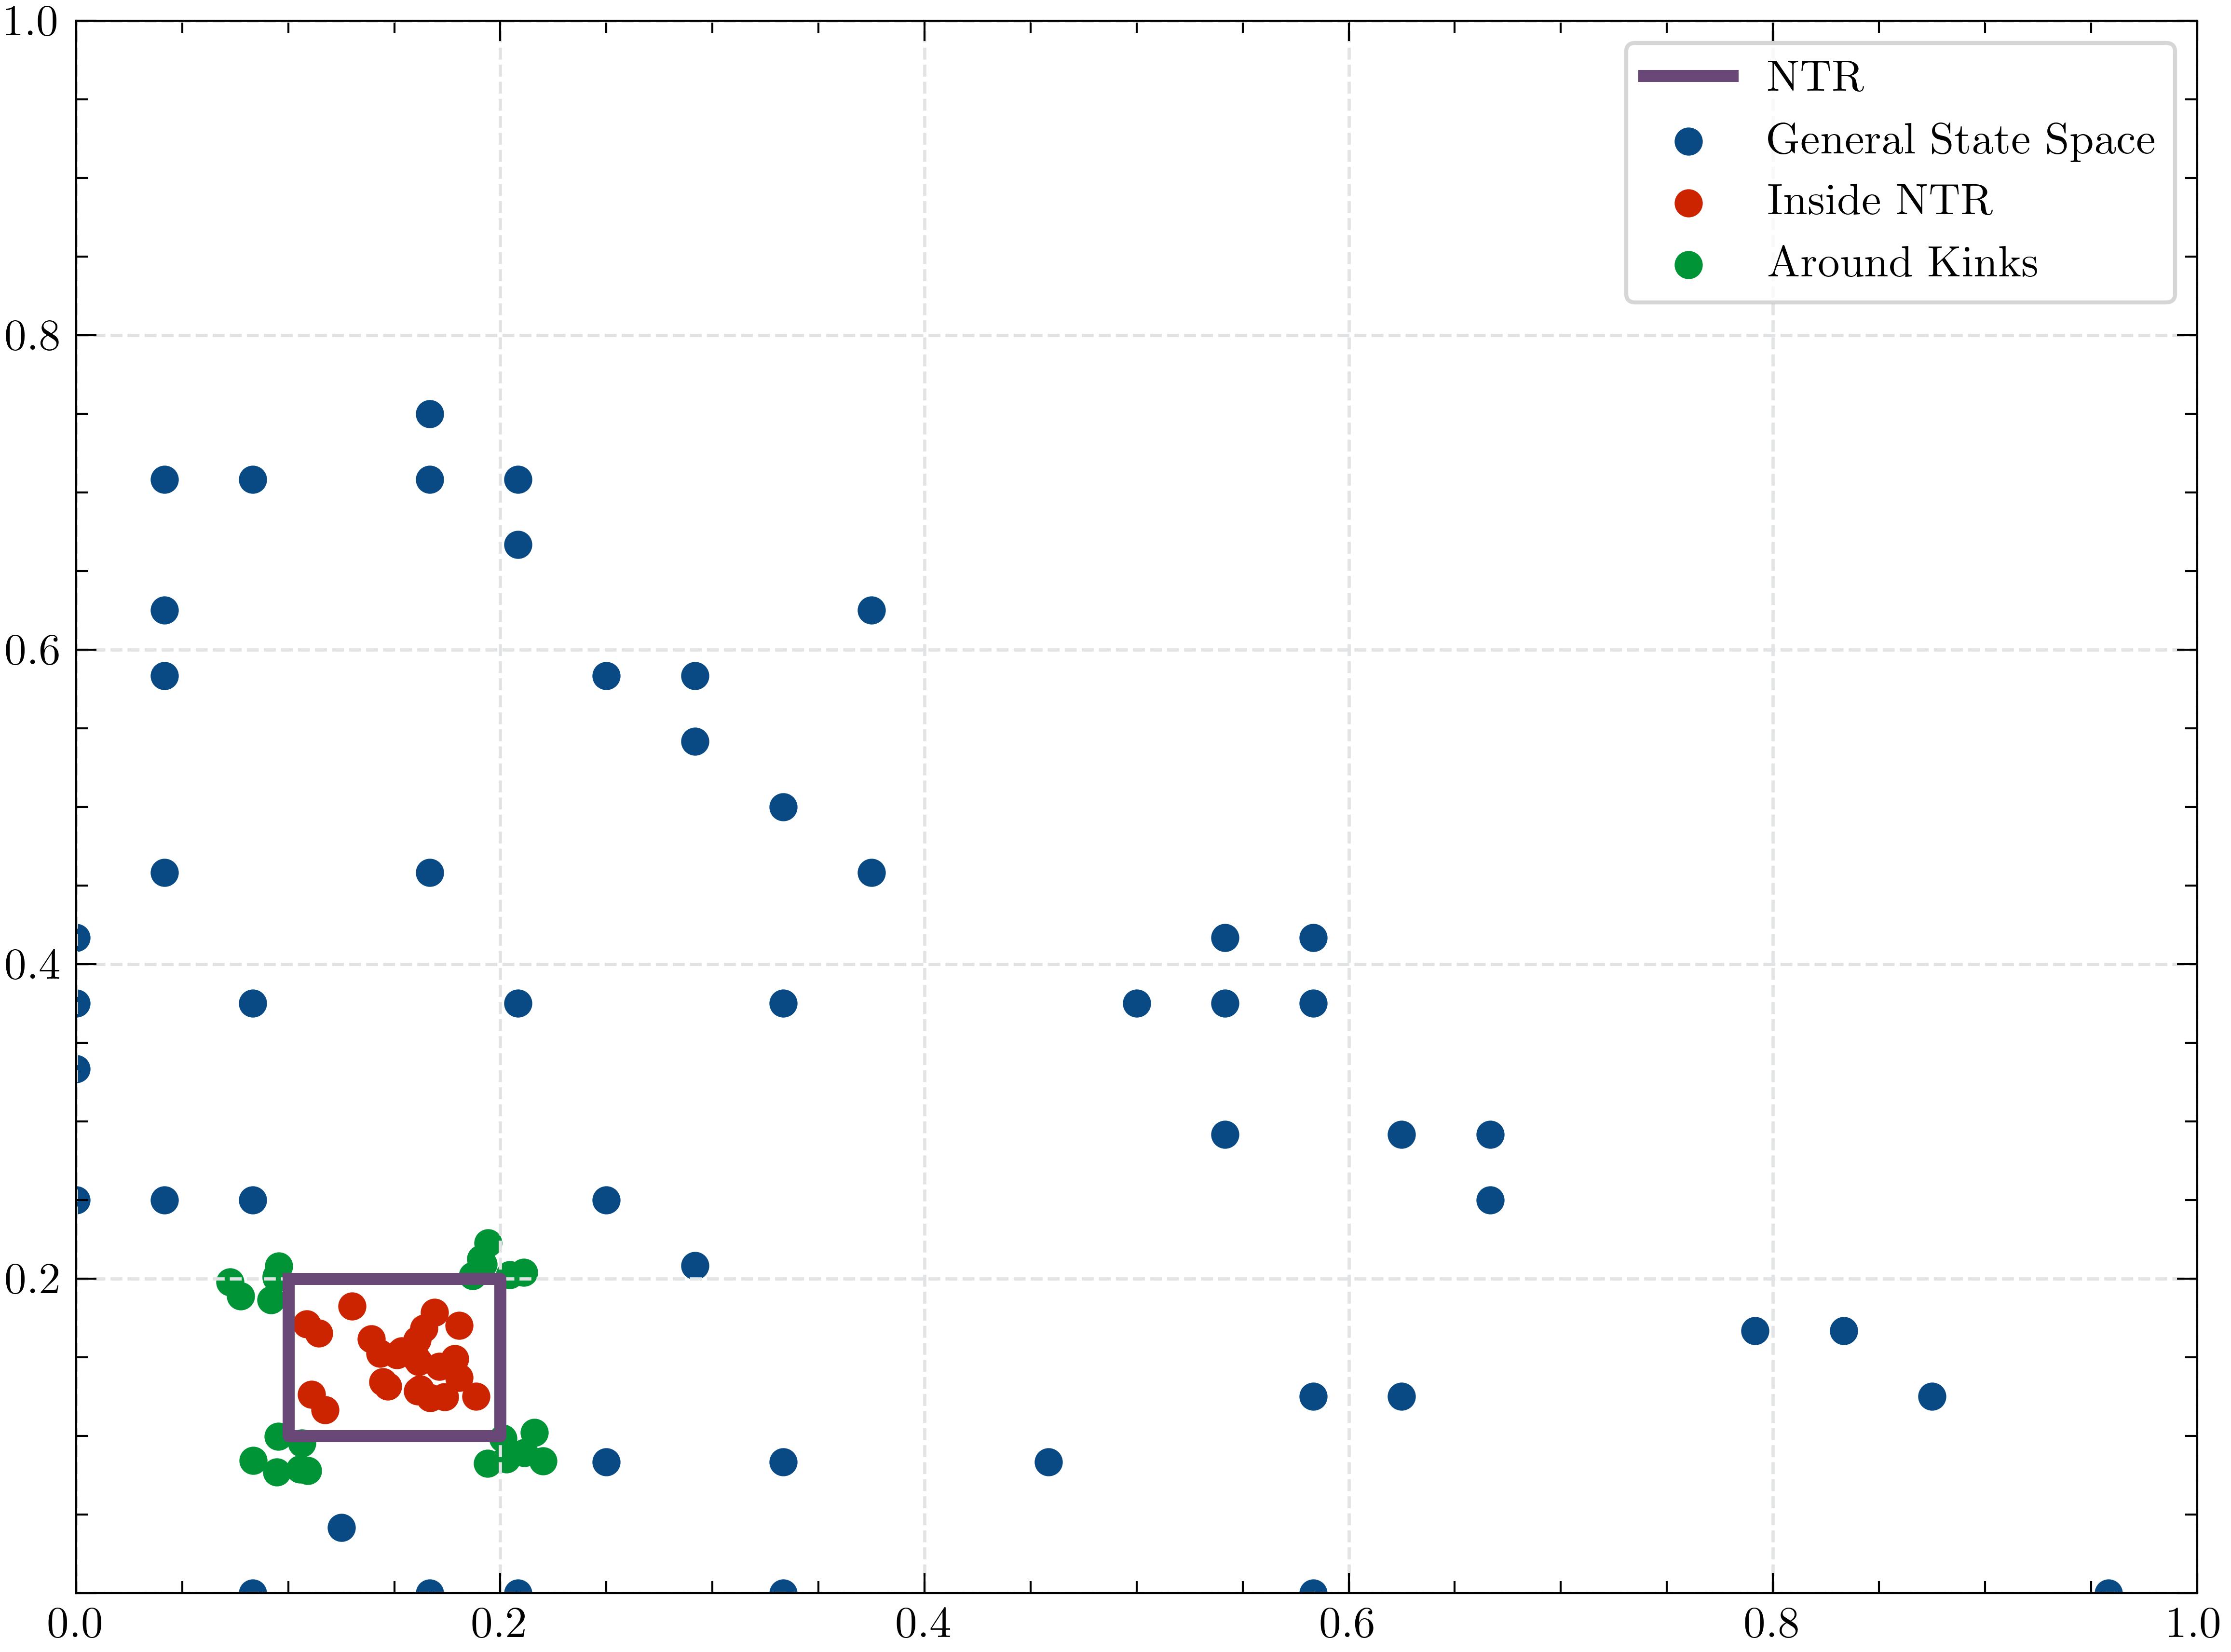
\includegraphics[scale=0.34]{designed_sampling_strategy.png}
  \end{center}
  \floatfoot{\textbf{Note:} Sample consists of $N=100$ points, with $51$ points in the general state space, $25$ points inside the NTR and $24$ points around the NTR kinks.}
  \end{figure}

\begin{figure}[h!]
  \begin{center}
  \caption{Zoom in on the NTR} 
  \label{fig: Zoom_Designed_sampling_strategy}
  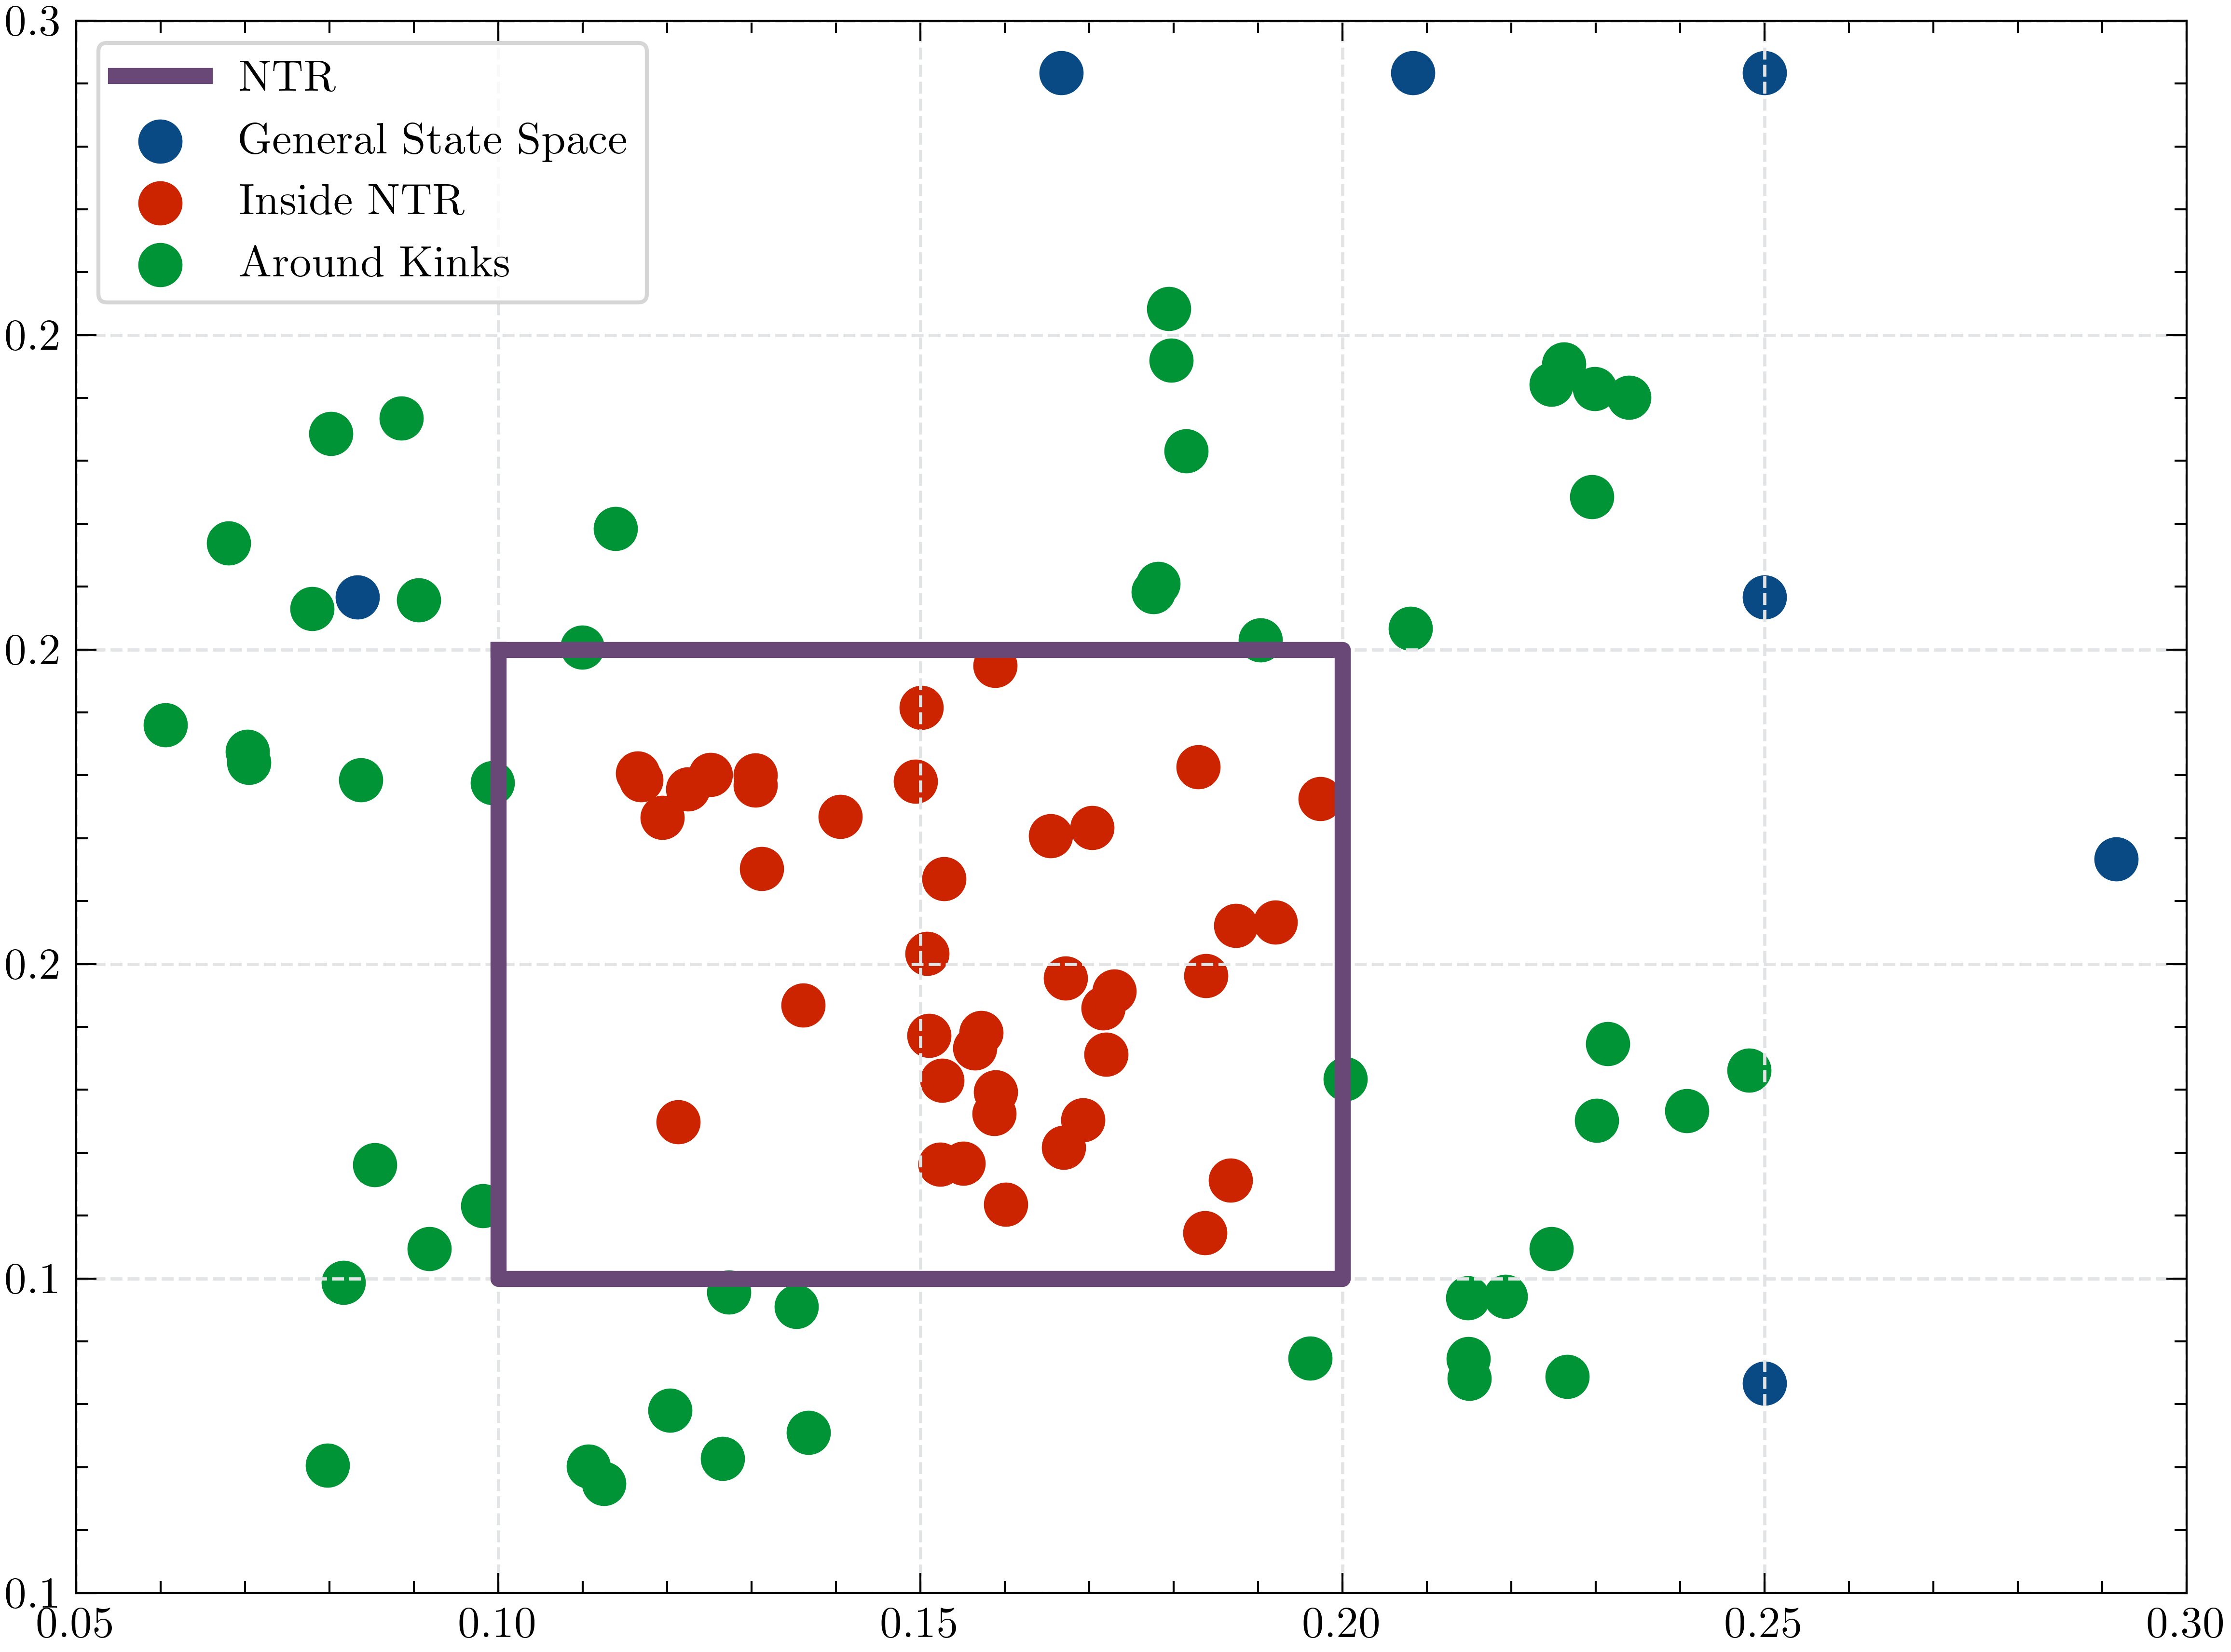
\includegraphics[scale=0.34]{zoomed_designed_sampling_strategy.png}
  \end{center}
  \floatfoot{\textbf{Note:} Sample consists of $N=100$ points, with $51$ points in the general state space, $25$ points inside the NTR and $24$ points around the NTR kinks.}
  \end{figure}

\subsection{Leveraging the no trade region} \label{Subsection: NTR-aproximation}
\subsection{Final solution algorithm} \label{Subsection: Algorithm}

\ifdefined\COMPILINGMAIN
% Main file is compiling this section, skip the end
\else
% \printbibliography
\end{document}
\fi